\chapter{Activity Based Computing}

In this chapter we will explain the activity-based paradigm further explained. We will explain why adaptation and awareness is important, and introduce two frameworks that will help us create an activity based client.

\section{Background}
As explained in the introduction, activity based computing is a new computer paradigm that moves focus from application based computer interaction into a higher level computational support for human activities. The paradigm has its outset in clinical work on hospitals, and seeks to aggregate resources to activities, instead of specific applications. An example of such an activity could be the development of our proof of concept. Opening an activity will cause the relevant services and resources to become available to the user, and allow to user to more easily switch between activities and all their associated services and resources. Figure \ref{fig:activitychart} shows an example of the activity "Proof-of-concept development", its associated services and their resources.

\begin{figure}[h!]
  \centering
    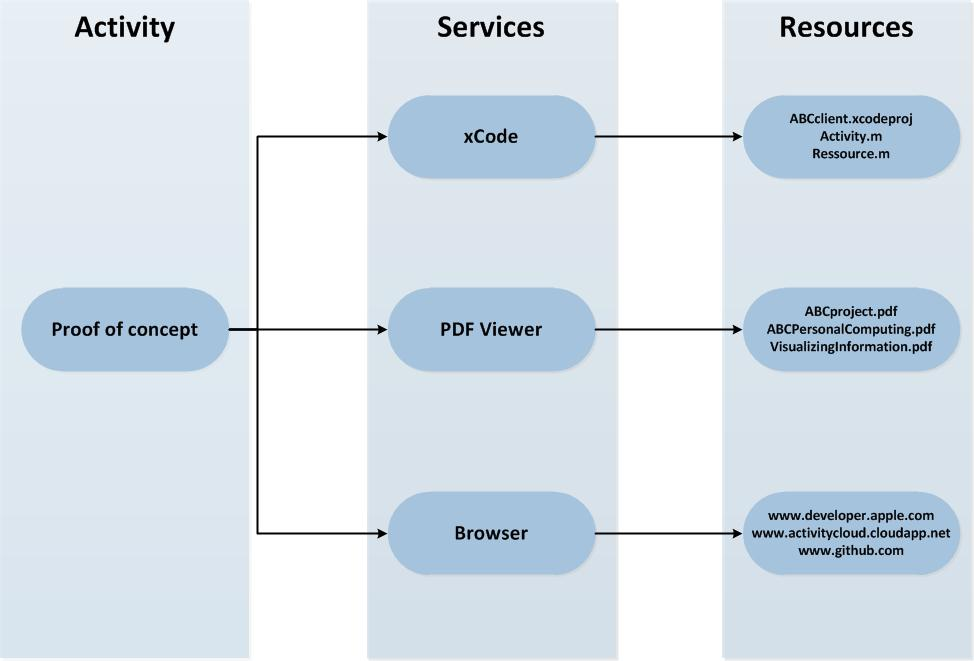
\includegraphics[scale=1.0]{ActivityChart}
  \caption{\emph{The "Proof of Concept" activity. Illustrates how an activity encapsulates its services and resources}}
  \label{fig:activitychart}
\end{figure}

\citet{bardram2011} identifies six principles that forms the basis of the activity based computing paradigm, being; \emph{Activity Centered}, \emph{Activity Suspend and Resume}, \emph{Activity Roaming}, \emph{Acitivty Adaptation}, \emph{Activity Sharing} and \emph{Activity Awareness}. Each of these will be further described in the following.

\begin{description}

	\item[1. Activity Centered] \hfill \\
	An Activity is a computational unit that encapsulates a set of services and their relevant resources. An activity therefore encapsulate digital software and data necessary for a user to carry out their work (activity).
	
	\item[2. Activity Suspend and Resume] \hfill \\
	This allows a user to alternate between several activities and support interruptions that requires the user to perform another task. This is done by suspending the current activity and resuming another.
	
	\item[3. Activity Roaming] \hfill \\
	This principle enables activities to be stored on an infrastructure, like a server, and allows for activities to be suspended on one device, and then resumed on another, to better support user mobility.
	
	\item[4. Activity Adaptation] \hfill \\
	An activity can be displayed and handled on very different devices, and should adapt to the resources available at the resumed devices. In this case resources could be CPU power, screen size and network bandwidth.
	
	\item[5. Activity Sharing] \hfill \\
	Focuses and deals with the collaborative aspect of activities. This principle states that activities are shared among collaborators that appear on a list of participants for any particular activity. If two or more participants engage resumes the same activity they will both be notified and engage in video and audio chat if possible.
		
	\item[6. Activity Awareness] \hfill \\
	Allows for an activity to be context aware, such that it adapts itself to its current environment and work context. This could be to i.e. adapting the user interface or changing activities and services based on where the device is located.

\end{description}

Implementing all of these features enables computational devices to better support human activities, and allow users to move away from the traditional document -and application centered model on a desktop computer. In this thesis we will focus on how to display activities on the iPad and how to adapt the interface to the orientation of the iPad, how to store activities in an infrastructure and how the iPad can be aware of its surroundings. In this chapter we will further explain the principle of adaptation and awareness.

\section{Activity Adaptation and Awareness}
One of the major challenges in supporting human activities in a computer environment, are when the human activities no longer applies to a stationary device. Many work environments requires the users to move around in order to complete an activity. An environment where this is especially difficult is in hospitals as addressed in \citet{bardram2009}, but even in a familiar environment like the IT-University, one is usually moving between 3 or 4 locations during a day. Usually when one is moving to a new location, the activities that are relevant to you changes, and thus one need not see all available activities, but only a subset of these. This requires the device to be able to detect the current location that the user is currently in, and to update the available activities. \citet{bardram2009} explains that it is necessary to find a way to notify the user about changes in the context, and that the list of activities has changed based on this new context. \citet{bardram2009} also argues that based on the evaluation with the clinical personnel, tablets were not deemed proper for mobile work situations based on some physical criteria. The personnel thought that the tablets were to large, meaning that they didnt fit in their large white-coat pockets and that they were to heavy to operate. The research were conducted back in 2009, which is before the iPad was launched, and compared to tablets that existed back then, the screen is slightly smaller, 9.7 inches compared to the 11-12 inches tablets had back then, which might make it possible to fit it into a pocket, and the weight has decreased a lot, from 1.5 - 2 kg's to rought 600 grams. Especially the decrease in the weight might again make the tablet a good device to use in mobile environments. And with the use of Activity Roaming principle, the user would probably not even need to carry it around, but just pick up a device at the desired location, to resume their last activity as \citet{bardram2009} argues.
\par\vspace{\baselineskip}
A second issue with mobility also found during evaluation by \citet{bardram2009} is that of changing screen sizes between devices. When a person moved from a device with a large screen like 1900×1600 to a smaller screen like 800x600, the saved states of each displayed service might not appear on the screen at all when resumed on a smaller device. This shows that it might not be feasible to have a similar implementation between devices with very different screen sizes. The iPad for example has a very distinct screen size, both in terms of physical size, but also in terms of resolution, so to try and imitate a work environment similar to a desktop computer would not be a good idea, because it is nothing like a desktop computer. One would therefore come up with a UI design that is different from a standard desktop UI, to eliminate the issues of positioning on the screen. It is also important to notice that a user would probably not use a small tablet computer for the same tasks that the user uses a large desktop computer for. For a tablet such as the iPad one could also take into account that the two orientations of the device could show a different UI, since it will move from a widescreen view to a portrait view, and thus make the UI more adaptable.

\section{ABC Framework}

